% Uncomment this to make slides with overlays:
%\documentclass[slides]{beamer}

% Uncomment these (but comment the above \documentclass line) to make handouts:
\documentclass[handout]{beamer}

% Uncomment these to have more than one slide per page
%\usepackage{pgfpages}
%\pgfpagesuselayout{2 on 1}[border shrink=5mm]
%\pgfpageslogicalpageoptions{1}{border code=\pgfusepath{stroke}}
%\pgfpageslogicalpageoptions{2}{border code=\pgfusepath{stroke}}

\usepackage[]{graphicx, color, hyperref}

\mode<presentation>
{
	%\usetheme[secheader]{Boadilla}
	%\usecolortheme[rgb={.835, .102,.169}]{structure}  
	\usetheme[width= 0cm]{Goettingen}
	%\setbeamercovered{transparent}
}
\setbeamertemplate{navigation symbols}{}
\setbeamertemplate{footline}[frame number]

\definecolor{blue2}{rgb}{0.278,0.278,0.729} 
\newcommand{\blue}[1]{\textcolor{blue2}{#1}}
\newcommand{\white}[1]{\textcolor{white}{#1}}
\newcommand{\red}[1]{\textcolor{red}{#1}}
\newcommand{\xbar}{\overline{x}}
\newcommand{\ybar}{\overline{y}}
\newcommand{\phat}{\widehat{p}}
\newcommand{\prob}{\mbox{Pr}}
\newcommand{\E}{\mathbb{E}}
\newcommand{\Var}{\mbox{Var}}
\newcommand{\cp}{\oplus}
\newcommand{\cm}{\circleddash}

\title{Lecture 11: Binomial and Poisson Random Variables}
\author{Chapter 3.3-3.5}
\date{}


\begin{document}
%------------------------------------------------------------------------------
\begin{frame}
\titlepage
\end{frame}
%------------------------------------------------------------------------------


%------------------------------------------------------------------------------
\begin{frame}[fragile]
\frametitle{Goals for Today}

Define
\begin{itemize}
\item Binomial random variables
\item Poisson random variables
\end{itemize}


\end{frame}
%------------------------------------------------------------------------------


%------------------------------------------------------------------------------
\begin{frame}
\frametitle{Binomial Distribution}

Say instead of $P(\mbox{1st W in 5th game})$, we want the probability that they win \blue{exactly one} out of the five games.  Five ways:

\pause\begin{center}
\begin{tabular}{c|ll}
Pattern & Probability & Equals\\
\hline
\blue{WLLLL} & $p \times (1-p)^4$ & $=p\times(1-p)^4$\\
\blue{LWLLL} & $(1-p) \times p \times (1-p)^3$ & $=p\times(1-p)^4$\\
\blue{LLWLL} & $(1-p)^2 \times p \times (1-p)^2$& $=p\times(1-p)^4$\\
\blue{LLLWL} & $(1-p)^3 \times p \times (1-p)$& $=p\times(1-p)^4$\\
\blue{LLLLW} & $(1-p)^4 \times p$& $=p\times(1-p)^4$\\
\end{tabular} 
\end{center}


\end{frame}
%------------------------------------------------------------------------------


%------------------------------------------------------------------------------
\begin{frame}
\frametitle{Binomial Distribution}

%
% Comment these
%
Each pattern has the same probability regardless of order by independence and there are 5 ways to \blue{choose} the pattern.  So

\vspace{0.25cm}

\begin{eqnarray*}
P(\mbox{exactly one win out of five}) &=& 5 \times p\times(1-p)^4\\
&=& 5 \times 0.4^4 \times 0.6 = 0.0768
\end{eqnarray*}

\end{frame}
%------------------------------------------------------------------------------



%------------------------------------------------------------------------------
\begin{frame}
\frametitle{Step Back... Example of $n$ choose $x$}
Say I give you $n=3$ balls labeled 1 thru 3.  How many different ways can you choose $x=2$ of them?  3 ways:

\[
(1, 2), \ (1, 3), \mbox{ and } \ (2, 3)
\]

\end{frame}
%------------------------------------------------------------------------------



%------------------------------------------------------------------------------
\begin{frame}
\frametitle{Step Back... $n$ choose $x$ in General}

%
% Comment these
%
Say I give you $n$ balls labeled 1 thru n.  How many different ways can you choose $x$ of them?  This is read \blue{n choose x}:

\[
{n \choose x} = \frac{n!}{x!(n-x)!}
\] 

\vspace{0.5cm}

In example: $n=3$ and $x=2$
\[
{3 \choose 2} = \frac{3!}{2!(3-2)!} = \frac{3 \times 2 \times 1}{(2 \times 1)(1)} = \frac{6}{2} = 3
\]

Note that $0!=1$

\end{frame}
%------------------------------------------------------------------------------


%------------------------------------------------------------------------------
\begin{frame}
\frametitle{Binomial Distribution}
%
% Comment these
%
Suppose the probability of a single trial being a success is $p$.  Let $X$ be the random number of successes observed in $n$ independent trials.  The probability of observing $x$ successes is:

\pause\begin{eqnarray*}
P(X=x) &=& {n \choose x} p^x (1-p)^{n-x}\\
&=& \frac{n!}{x!(n-x)!}p^x (1-p)^{n-x}
\end{eqnarray*}

\pause The mean, variance, and SD are:
\[
\mu = np \hspace{1cm} \sigma^2 = np(1-p) \hspace{1cm} \sigma = \sqrt{np(1-p)}
\]

\end{frame}
%------------------------------------------------------------------------------


%------------------------------------------------------------------------------
\begin{frame}
\frametitle{Conditions for Binomial Distribution}

%
% Comment these
%
\begin{enumerate}
\pause\item The trials are independent.
\pause\item The number of trials $n$ is fixed
\pause\item Each trial outcome can be classified as a failure or a success
\pause\item The probability of a success $p$ is the same for each trial
\end{enumerate}

\end{frame}
%------------------------------------------------------------------------------


%------------------------------------------------------------------------------
\begin{frame}
\frametitle{Back to Soccer Example}
Probability of exactly one win?

\begin{center}
\begin{tabular}{c|ll}
Pattern & Probability & Equals\\
\hline
\blue{WLLLL} & $p \times (1-p)^4$ & $=p\times(1-p)^4$\\
\blue{LWLLL} & $(1-p) \times p \times (1-p)^3$ & $=p\times(1-p)^4$\\
\blue{LLWLL} & $(1-p)^2 \times p \times (1-p)^2$& $=p\times(1-p)^4$\\
\blue{LLLWL} & $(1-p)^3 \times p \times (1-p)$& $=p\times(1-p)^4$\\
\blue{LLLLW} & $(1-p)^4 \times p$& $=p\times(1-p)^4$\\
\end{tabular} 
\end{center}

%
% Comment these
%
\pause Letting a win be a ``success'':
\begin{eqnarray*}
P(X=1) &=& {n \choose x} p^x (1-p)^{n-x} = \frac{5!}{1!\times4!} 0.6 \times 0.4^4\\
&=& 5 \times  0.6 \times 0.4^4 = 0.0768
\end{eqnarray*}

\end{frame}
%------------------------------------------------------------------------------


%------------------------------------------------------------------------------
\begin{frame}
\frametitle{Back to Soccer Example}
%
% Comment these
%
What is the probability that they win all their games!  i.e. $X=5$:
\pause \begin{eqnarray*}
P(X=5) &=& {n \choose x} p^x (1-p)^{n-x} = {5 \choose 5} 0.6^5 (1-0.6)^{0}\\
&=& \frac{5!}{5!\times 0!} 0.6^5 \times 1 = 0.08
\end{eqnarray*}

\vspace{0.75cm}

\pause What is the probability that they at win at least one game?
\pause \begin{eqnarray*}
P(X\geq 1) &=& P(X=1) + \ldots + P(X=5) \\
&=& 1 - P(X=0)\\
&=& 1 -  \frac{5!}{0!\times 5!} 0.6^0 \times 0.4^5 = 1 - 0.01024\\
&=& 0.98976
\end{eqnarray*}

\end{frame}
%------------------------------------------------------------------------------


%values <- data.frame(
%  x = c(0:5),
%  y = dbinom(c(0:5), size=5, prob=0.6)
%)
%ggplot(values, aes(x=as.factor(x), y=y)) + geom_bar(stat="identity") +
%  xlab("x = # of successes") +
%  ylab("P(X=x)")
%ggsave("./Lec11 Binomial and Poisson/figure/bin.pdf")
%------------------------------------------------------------------------------
\begin{frame}
\frametitle{Back to Soccer Example}

\begin{center}
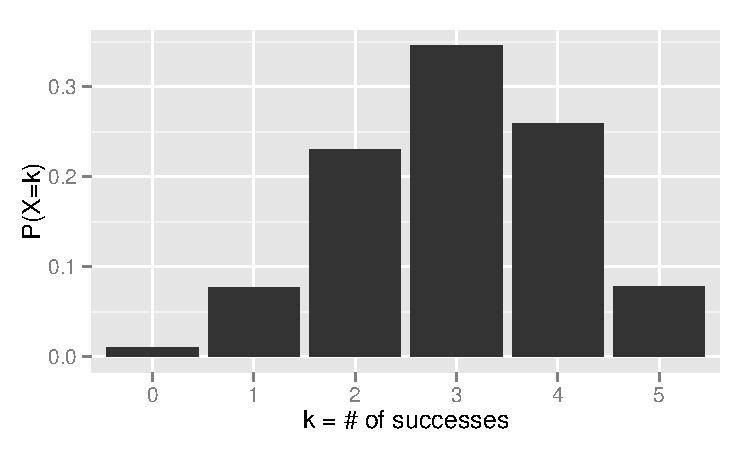
\includegraphics[width=\textwidth]{figure/bin.pdf}
\end{center}

\end{frame}
%------------------------------------------------------------------------------


%------------------------------------------------------------------------------
\begin{frame}
\frametitle{Poisson Distribution}

Say you want to count the number of rare events in a large population over a unit of time.  Ex:
\begin{itemize}
\pause \item \# of car accidents at an intersection on a given week
\pause \item \# of ambulance calls on any given day in Portland
\pause \item \# of soldiers in the Prussian army killed accidentally by horse kick from 1875 to 1894
\end{itemize}

\vskip 0.25cm

\pause The \blue{Poisson distribution} helps us model such counts.

\end{frame}
%------------------------------------------------------------------------------


%------------------------------------------------------------------------------
\begin{frame}
\frametitle{Poisson Distribution}
%
% Comment these
%
A random number $X$ of the count of the number of events follows a Poisson distribution with rate $\lambda$
\[
    P(\mbox{we observe x rare events}) = P(X=x) = \frac{\lambda^x e^{-\lambda}}{x!}
\]
\pause where x may take a value 0, 1, 2, \ldots where $e \approx 2.718$.

\vspace{0.5cm}

\pause The mean and SD are $\lambda$ and $\sqrt{\lambda}$.

\end{frame}
%------------------------------------------------------------------------------


%------------------------------------------------------------------------------
\begin{frame}
\frametitle{Conditions for Poisson Distribution}

%
% Comment these
%
A random variable \blue{may} be Poisson distributed if

\begin{enumerate}
\pause\item The event in question is rare
\pause\item The population is large
\pause\item The events occur independently of each other
\end{enumerate}

\end{frame}
%------------------------------------------------------------------------------


%------------------------------------------------------------------------------
\begin{frame}
\frametitle{Exercise 3.47 on Page 158}
%
% Comment these
%
A coffee shop serves an average of 75 customers per hour during the morning rush.  Let $X$ be the (random) number of customers that the coffee shop serves in one hour at this time of the day.  

\vspace{0.5cm}

What is the probability $X=70$?

\end{frame}
%------------------------------------------------------------------------------


%------------------------------------------------------------------------------
\begin{frame}
\frametitle{Exercise 3.47 on Page 158}
%
% Comment these
%
In this case, $\lambda=75$ is the rate
\[
P(X=70) = \frac{75^{70} e^{-75}}{70!} = 0.040
\]

\pause\vspace{0.25cm}

We can do this in R via {\tt dpois(x=70, lambda=75)} in {\tt R}

\end{frame}
%------------------------------------------------------------------------------


%------------------------------------------------------------------------------
\begin{frame}[fragile]
\frametitle{Next Time}

Chapter 4:  Foundations for Inference
\begin{itemize}
\item Variability in estimates $\overline{x}$, $\widehat{p}$, etc.
\item In fact, we can associate a \blue{distribution} to these estimates
\end{itemize}


\end{frame}
%------------------------------------------------------------------------------



\end{document}


